\documentclass[a4paper,12pt]{report}
\usepackage[utf8]{inputenc}
\usepackage[T1]{fontenc}
\usepackage[ngerman]{babel}

\usepackage{listings}
\usepackage{amsmath}
\usepackage{hyperref}
\usepackage{xcolor}
\usepackage{parskip}
\usepackage{tcolorbox}
\usepackage{placeins}
\usepackage{graphicx}
%\graphicspath{{images/}}


\lstdefinestyle{java}{
  language=Java,
  basicstyle=\ttfamily\small,
  keywordstyle=\color{blue}\bfseries,
  stringstyle=\color{red},
  commentstyle=\color{gray}\itshape,
  numbers=left,
  numberstyle=\tiny\color{gray},
  stepnumber=1,
  numbersep=5pt,
  tabsize=2,
  showstringspaces=false,
  breaklines=true,
  frame=single
}

\lstset{style=java}

\hypersetup{
    colorlinks=true,
    linkcolor=black,
    urlcolor=blue,
    citecolor=black,
    pdfborder={0 0 0}
}

\usepackage{caption}
\usepackage{geometry}
\usepackage{lmodern}
\geometry{left=3cm,right=2.5cm,top=2.5cm,bottom=2.5cm}

% Titelblatt
\begin{document}

\begin{titlepage}
    \centering
    \vspace*{3cm}
    {\Huge \textbf{Dokumentation der praktischen Arbeit}}\\[2cm]
    {\large zur Prüfung zum \\ Mathematisch-technischen Softwareentwickler}\\[2cm]
    {\Large \textbf{Thema: Simulation von Verkehrsflüssen}}\\[1cm]
    {16.05.2025}\\[5cm]
    {Daniel Ebel}\\[2cm]
    Prüflingsnummer: 101 20015\\[0.5cm]
    Bearbeitungszeitraum: 12.05.2025 - 16.05.2025\\[0.5cm]
    Programmiersprache: Java\\[0.5cm]
    Ausbildungsort: INFORM GmbH
\end{titlepage}

% Eigenständigkeitserklärung
\chapter*{Eigenständigkeitserklärung}
Ich erkläre, dass das vorliegende Prüfprodukt von mir selbstständig erstellt wurde.
Die als Arbeitshilfe genutzten Unterlagen sind in der Arbeit vollständig aufgeführt.
Ich versichere, dass der vorgelegte Ausdruck mit dem Inhalt der von mir erstellten digitalen Version identisch ist.
Weder ganz noch in Teilen wurde die Arbeit bereits als Prüfungsleistung vorgelegt.
Mir ist bewusst, dass jedes Zuwiderhandeln als Täuschungsversuch zu gelten hat, der die Anerkennung als Prüfungsleistung ausschließt.

\vspace{2cm}

Aachen, 16.05.2025

\vspace{1cm}

\noindent\rule{7cm}{0.4pt}\\
Unterschrift

\tableofcontents
%\listoffigures

\chapter{Einleitung}
Zur Bewertung von Verkehrsflüssen und zur Identifikation kritischer Straßenabschnitte soll eine Verkehrssimulation entwickelt werden.
Grundlage der Simulation ist eine Eingabedatei mit Einfalls- und Kreuzungspunkten sowie ein definierter Simulationszeitraum.
Fahrzeuge treten an Einfallspunkten mit bestimmten Taktraten auf, bewegen sich mit zufälliger,
individuell festgelegter Geschwindigkeit durch das Netz und treffen an Kreuzungen zufallsbasiert Abbiegeentscheidungen gemäß festgelegter Wahrscheinlichkeiten.

Die Eingabe erfolgt über eine Textdatei mit folgendem Beispielinhalt:

\begin{lstlisting}
# Beispielhausen
Zeitraum:
50 1

Einfallspunkte:
A 0 0 B 2
C 0 2 B 5
D 4 0 E 3
F 4 2 E 2
G 5 1 E 3

Kreuzungen:
B 0 1 A 20 C 30 E 50
E 4 1 D 20 F 20 G 10 B 50
\end{lstlisting}

Die erste Zeile gibt einen Kommentar wieder.
Danach folgen der Simulationszeitraum (hier 50 Sekunden mit Ausgaben alle 1 Sekunde),
gefolgt von Einfallspunkten. Jeder Einfallspunkt enthält Position, Zielkreuzung und Taktzeit.
Anschließend werden Kreuzungen definiert,
die jeweils eingehende Straßen mit Richtungsverteilungen enthalten.

Ziel der Simulation ist es, Fahrzeugbewegungen zu modellieren,
deren Positionen für jeden Zeitschritt in einer Datei ausgegeben und mit einem Visualisierungstool dargestellt werden.
Zusätzlich werden für jede Straße statistische Kenngrößen wie kumulierte Fahrzeuganzahl und maximale Streckenauslastung berechnet.

\chapter{Aufgabenanalyse}
\section{Beschreibung Eingabedatei}

Die Eingabedatei muss UTF-8-kodiert sein;
anderenfalls wird eine Exception mit der Meldung „Eingabedatei ist nicht UTF-8 kodiert“ ausgelöst.
Die Datei gliedert sich in exakt drei Abschnitte: Zeitraum:, Einfallspunkte: und Kreuzungen:.
Jeder Abschnitt darf höchstens einmal vorkommen – doppelte Abschnitte führen zu einem Abbruch mit einer spezifischen Fehlermeldung.

Im Abschnitt Zeitraum: werden zwei Parameter erwartet: die Gesamtdauer der Simulation in Sekunden (maxTime) sowie die Taktfrequenz (clockrate),
also das Intervall in Sekunden, in dem Fahrzeuge generiert werden.
Beide Werte müssen positive Ganzzahlen sein. maxTime darf dabei 24 Stunden (86.400 Sekunden) nicht überschreiten.
Ein Eintrag wie z.,B. „50.0“ würde eine Fehlermeldung hervorrufen,
da Dezimalzahlen nicht erlaubt sind. Auch muss clockrate kleiner oder gleich maxTime sein.

Der Abschnitt Einfallspunkte: definiert Punkte,
an denen Fahrzeuge in das System eintreten.
Jede Zeile folgt dem Format Name X Y Ziel Takt. 
abei dürfen Namen maximal 100 Zeichen lang sein und nicht doppelt vorkommen.
Die Koordinaten X und Y müssen Gleitkommazahlen im Bereich von -1000 bis +1000 sein.
Zudem wird geprüft, dass kein Punkt näher als 0{,}1 Einheiten (entspricht 10 Metern) zu einem bereits definierten Punkt liegt.
Als Ziel wird eine Kreuzung angegeben, zu der das erste Fahrzeug weitergeleitet wird.
Der Takt bestimmt die Häufigkeit der Fahrzeuggenerierung in Sekunden und muss eine positive ganze Zahl sein.

Im Abschnitt Kreuzungen: wird jede Zeile im Format Name X Y Ziel1 Anteil1 Ziel2 Anteil2 ... erwartet.
Auch hier sind Namen auf 100 Zeichen begrenzt und dürfen nicht mehrfach vorkommen.
Die Ziel-Anteil-Paare müssen mindestens zweimal vorkommen,
wobei die Anzahl der Teile ungerade sein muss (wegen Name, X und Y zu Beginn).
Der Anteil (relative Wahrscheinlichkeit) muss als Dezimalzahl mit Punkt angegeben sein und zwischen $10^6$ und $10^{-6}$ liegen.
Auch hier dürfen Koordinaten nicht zu nahe beieinanderliegen.

Orte dürfen nicht gleichzeitig Einfallspunkte und Kreuzungen sein. Zudem müssen alle in Einfallspunkten oder Kreuzungen genannten Zielorte tatsächlich existieren – entweder als Kreuzung oder als anderer Einfallspunkt.

% \begin{figure}[h!]
%     \centering
%     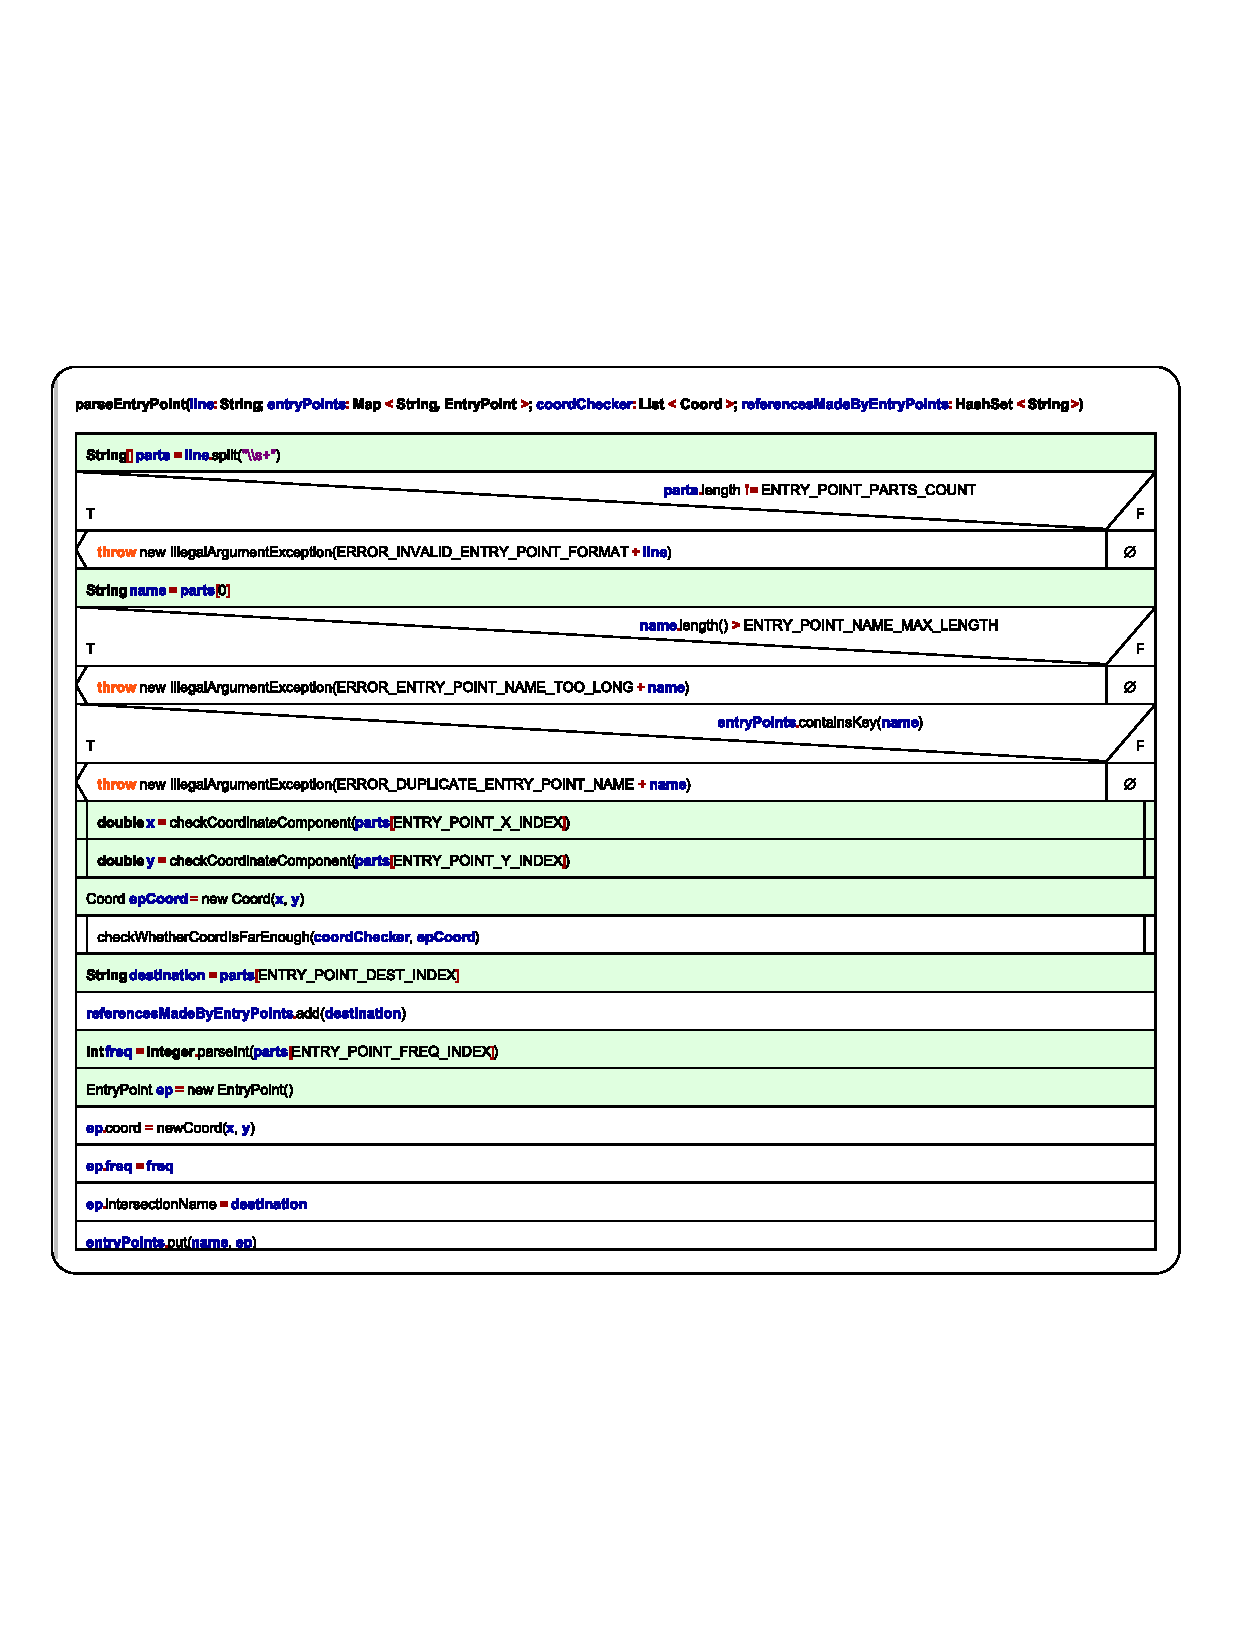
\includegraphics[width=0.8\textwidth]{nassis/TextFileReader/parseEntryPoint-4.pdf}
%     \caption{Example caption}
%     \label{fig:example}
% \end{figure}


\chapter{Verfahrensbeschreibung}

\section{Einlesen}

Die Klasse \texttt{TextFileReader} ist für das strukturierte Einlesen und Validieren der Eingabedatei zuständig.
Sie implementiert das Interface \texttt{Reader} und liefert mit der Methode \texttt{read()} ein vollständig initialisiertes \texttt{CityDTO}-Objekt,
das alle für die Simulation notwendigen Daten kapselt.

Der Leseprozess beginnt mit einer Prüfung der Dateiexistenz sowie der korrekten UTF-8-Kodierung.
Anschließend wird die Datei zeilenweise eingelesen. Kommentare (durch \texttt{\#} eingeleitet) werden entfernt,
leere Zeilen ignoriert. Die Datei ist in drei klar strukturierte Abschnitte gegliedert:

\begin{itemize}
  \item \textbf{Zeitraum:} Enthält zwei ganzzahlige Werte:
  \begin{itemize}
    \item \texttt{maxTime} -- Die gesamte Simulationsdauer in Sekunden.
    \item \texttt{clockRate} -- Das Intervall in Sekunden, in dem der Zustand aller Fahrzeuge gespeichert wird.
  \end{itemize}
  Es wird sichergestellt, dass beide Werte gültige positive Ganzzahlen sind. Dezimalzahlen und ungültige Werte führen zu klaren Fehlermeldungen.

 

\begin{figure}[h!]
    \centering
    \caption{Zeitraum Prüfmethoden in Nassi-Shneiderman-Diagrammen dargestellt:}
    \makebox[\textwidth][c]{\includegraphics[width=1.3\textwidth]{nassis/TextFileReader/timeSpanChecks.pdf}}
\end{figure}

\clearpage

  \item \textbf{Einfallspunkte:} Jede Zeile beschreibt einen Einfallspunkt im Format:
  \begin{center}
    \texttt{<Name> <x> <y> <Zielkreuzung> <Frequenz>}
  \end{center}
  Dabei stehen \texttt{x} und \texttt{y} für die Koordinaten, \texttt{Zielkreuzung} für das Ziel neu erzeugter Fahrzeuge,
  und \texttt{Frequenz} für das Erzeugungsintervall.
  Es wird validiert, dass:
  \begin{itemize}
    \item jeder Name eindeutig ist,
    \item die Zielkreuzung später im Kreuzungsabschnitt existiert,
    \item Koordinaten einen Mindestabstand (0{,}1 Einheiten) zueinander einhalten,
    \item die Frequenz eine positive Ganzzahl ist.
  \end{itemize}
  Jeder gültige Eintrag wird als \texttt{EntryPoint}-Objekt gespeichert.

  Einfallspunkt Parsemethode in Nassi-Shneiderman-Diagramm (bitte reinzoomen):
  \vspace{-1.5cm} 
  \FloatBarrier
  \begin{figure}[h!]
    \vspace{-1.5cm} 
    \centering
    %\caption{Einfallspunkt Parsemethode in Nassi-Shneiderman-Diagramm:}
    \makebox[\textwidth][c]{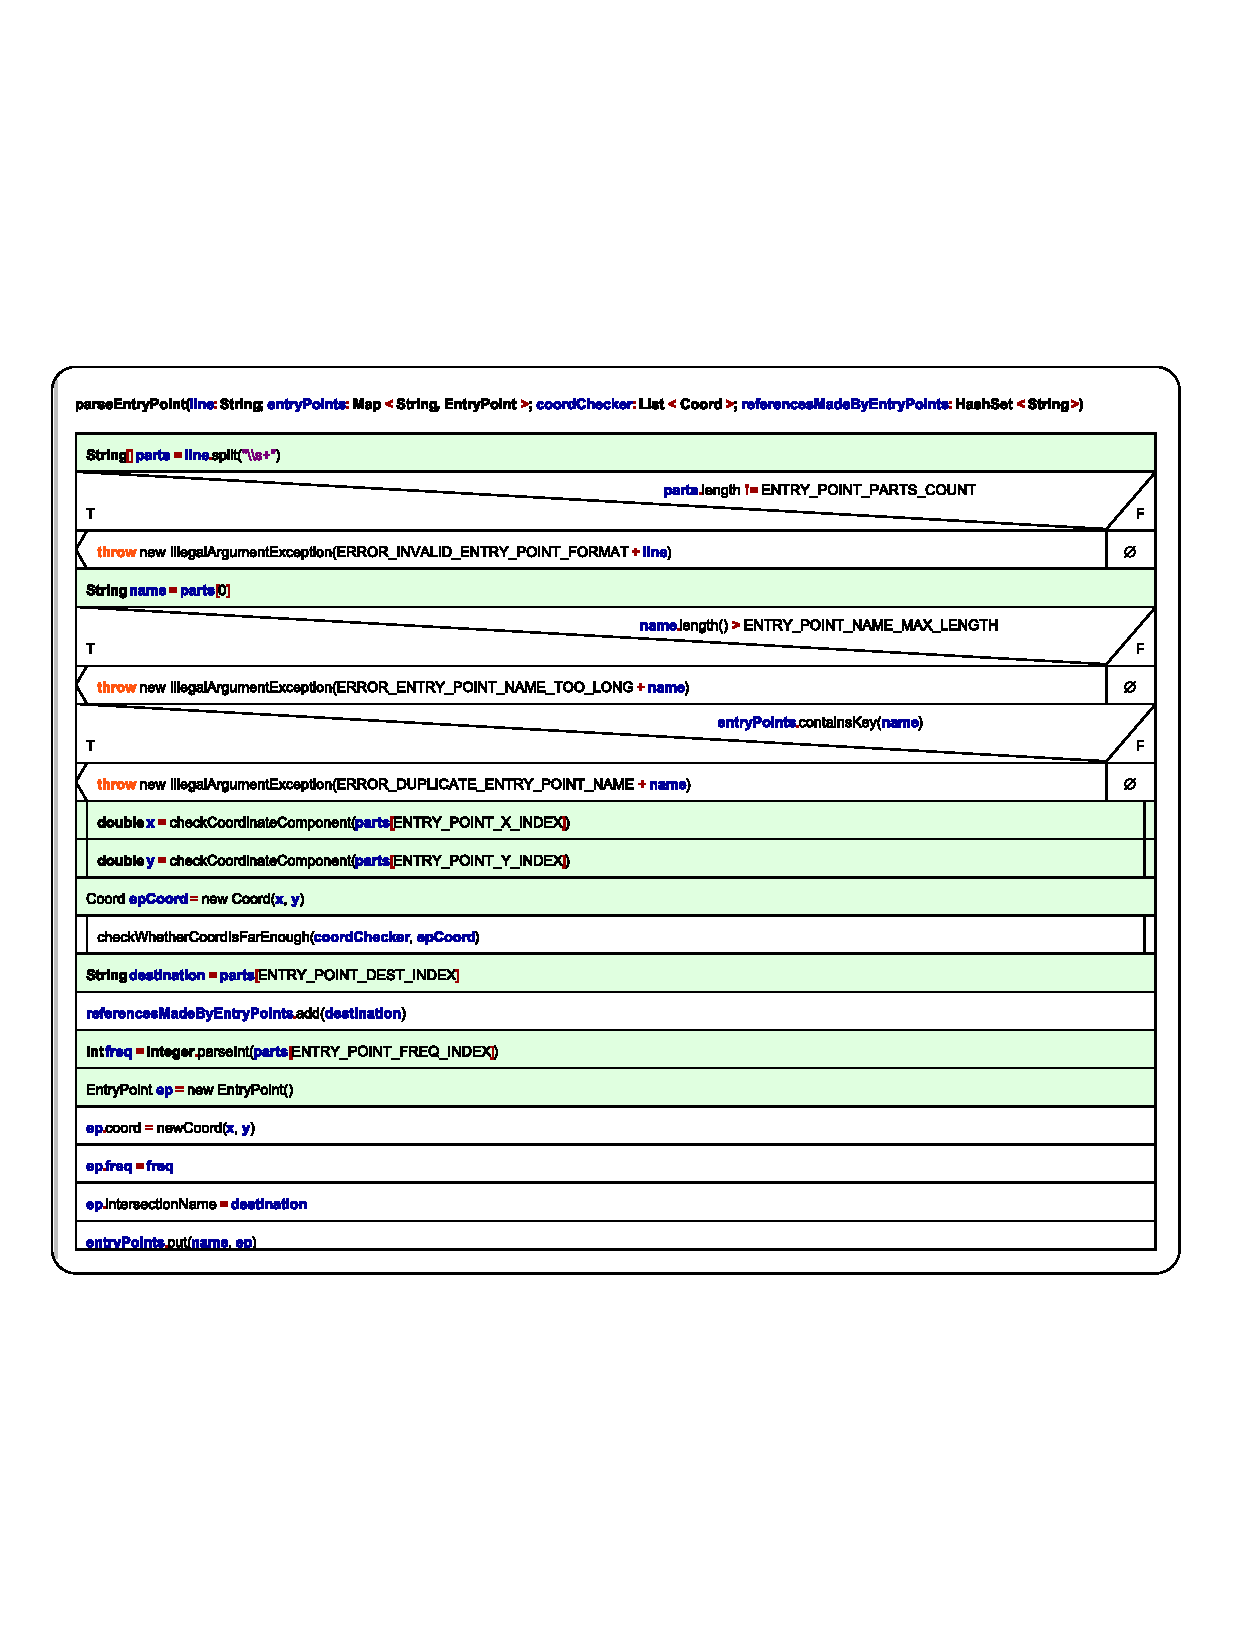
\includegraphics[width=0.9\textwidth]{nassis/TextFileReader/parseEntryPoint-4.pdf}}
\end{figure}

\clearpage

  \item \textbf{Kreuzungen:} Jede Zeile definiert eine Kreuzung und deren ausgehende Kanten:
  \begin{center}
    \texttt{<Name> <x> <y> <Ziel1> <Anteil1> <Ziel2> <Anteil2> ...}
  \end{center}
  Dabei werden:
  \begin{itemize}
    \item Koordinaten (\texttt{x}, \texttt{y}) eingelesen,
    \item Zielorte mit zugehörigen relativen Wahrscheinlichkeiten versehen,
    \item Wahrscheinlichkeiten automatisch normalisiert.
  \end{itemize}
Für jede Verbindung wird ein \texttt{DirectedEdge} (inklusive Gegenrichtung) angelegt.
Die zugehörigen statistischen Informationen werden in einem \texttt{DirectedEdgeInfo}-Objekt gespeichert.
Jede Kreuzung wird als \texttt{Intersection}-Objekt abgelegt.

Kreuzungs Parsemethode in Nassi-Shneiderman-Diagramm (bitte reinzoomen):
  \vspace{-4.5cm}
\end{itemize}
\FloatBarrier
\begin{figure}[h!]
    \vspace{-1.5cm} 
    \centering
    %\caption{Einfallspunkt Parsemethode in Nassi-Shneiderman-Diagramm:}
    \makebox[\textwidth][c]{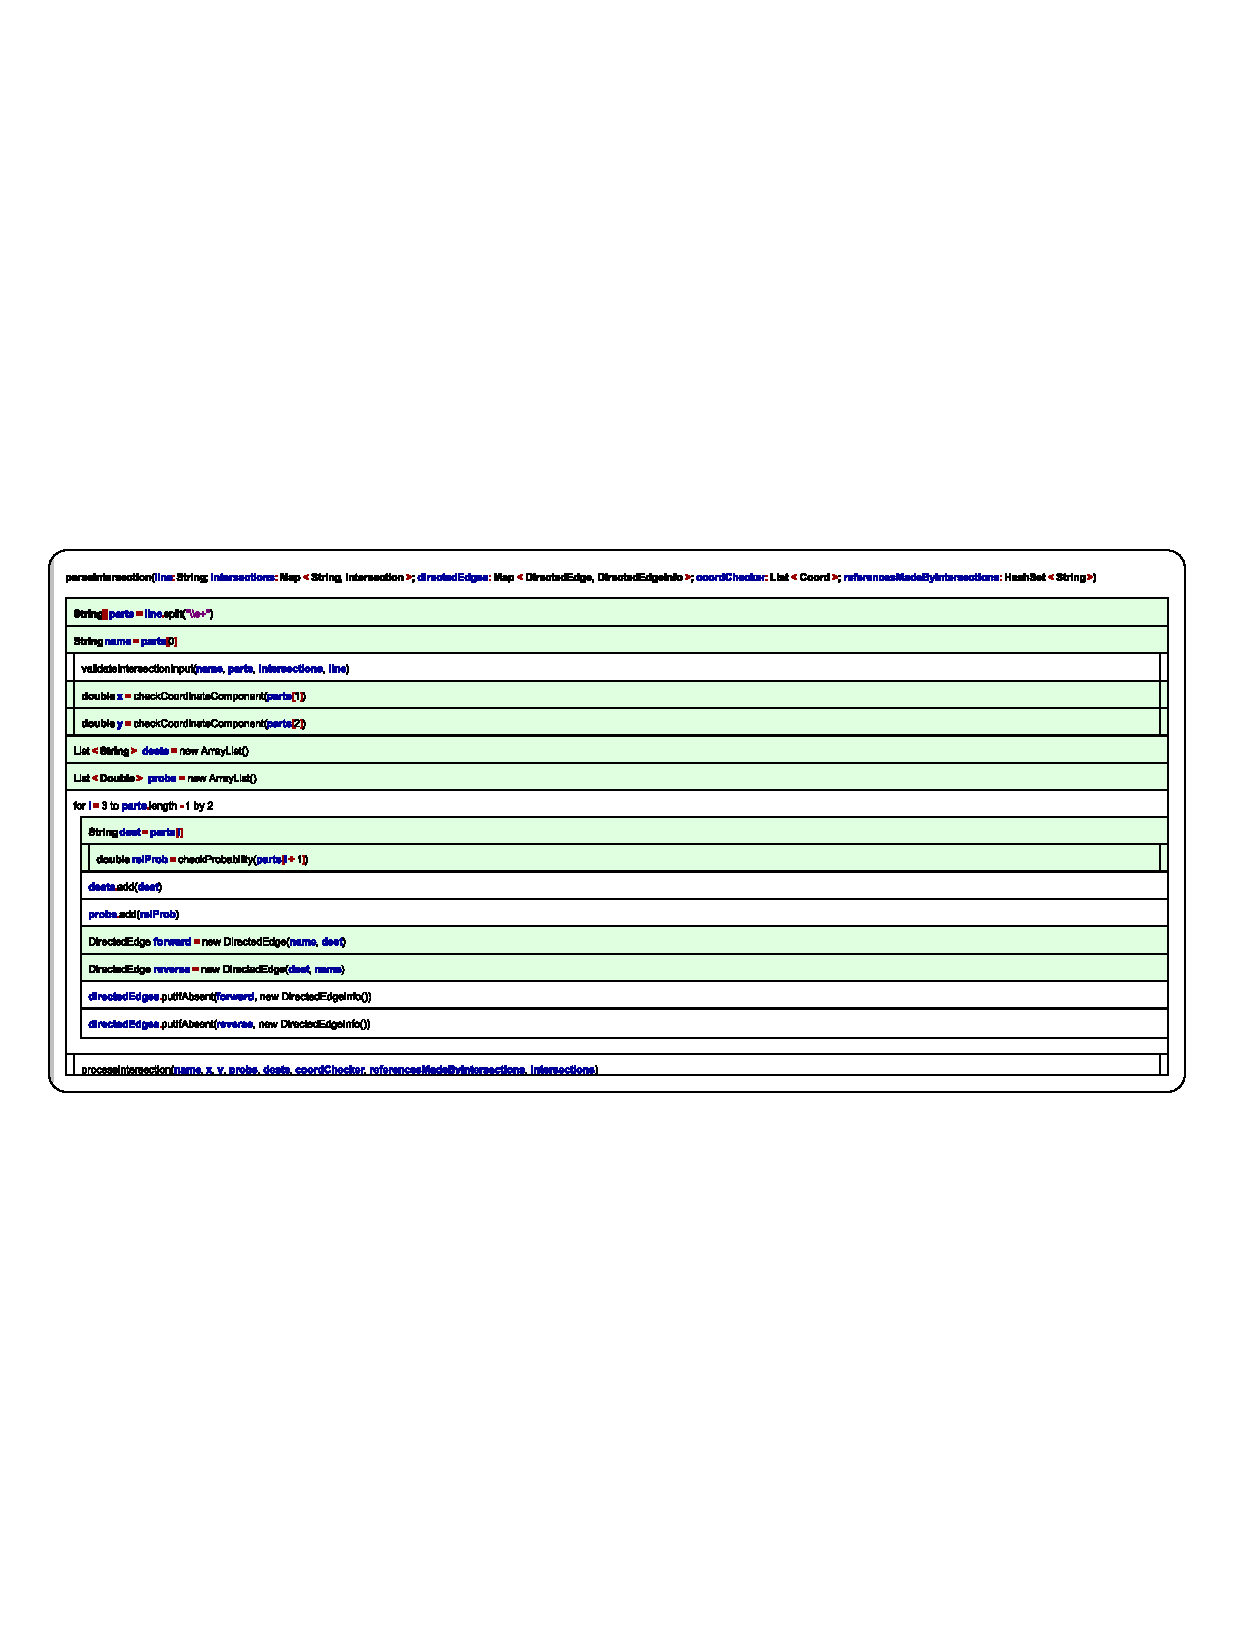
\includegraphics[width=1.11\textwidth]{nassis/TextFileReader/parseIntersection-5.pdf}}
\end{figure}

\clearpage

Nach Abschluss des Parsings werden verschiedene Konsistenzprüfungen durchgeführt:
\begin{itemize}
  \item Einfallspunkte und Kreuzungen dürfen nicht überlappen,
  \item Alle referenzierten Orte müssen existieren,
  \item Wahrscheinlichkeiten und Koordinatenwerte müssen im zulässigen Bereich liegen.
\end{itemize}

Abschließend werden alle Daten in ein \texttt{CityDTO}-Objekt überführt,
das als Grundlage für die Initialisierung der Simulation dient.

Auf der folgenden Seite lässt sich in das Nassi-Shneiderman Meisterwerk der, das \texttt{CityDTO} erzeugenden read-Methode hineinzoomen.
\begin{tcolorbox}[colback=blue!5!white, colframe=blue!75!black, title=Hinweis]
In den folgenden Nassi-Shneiderman-Diagrammen sind Java \texttt{try-with-resource}-Statements aufgrund von 
Limitationen der Nassi-Shneiderman-Diagramm-Erstellungssoftware \emph{Structorizer} wie folgt dargestellt:
\begin{verbatim}
var br: BufferedReader = null
try
...
br =
catch e
\end{verbatim}
\end{tcolorbox}

\clearpage
\FloatBarrier
\begin{figure}[h!]
    \vspace{-1.5cm} 
    \centering
    %\caption{Einfallspunkt Parsemethode in Nassi-Shneiderman-Diagramm:}
    \makebox[\textwidth][c]{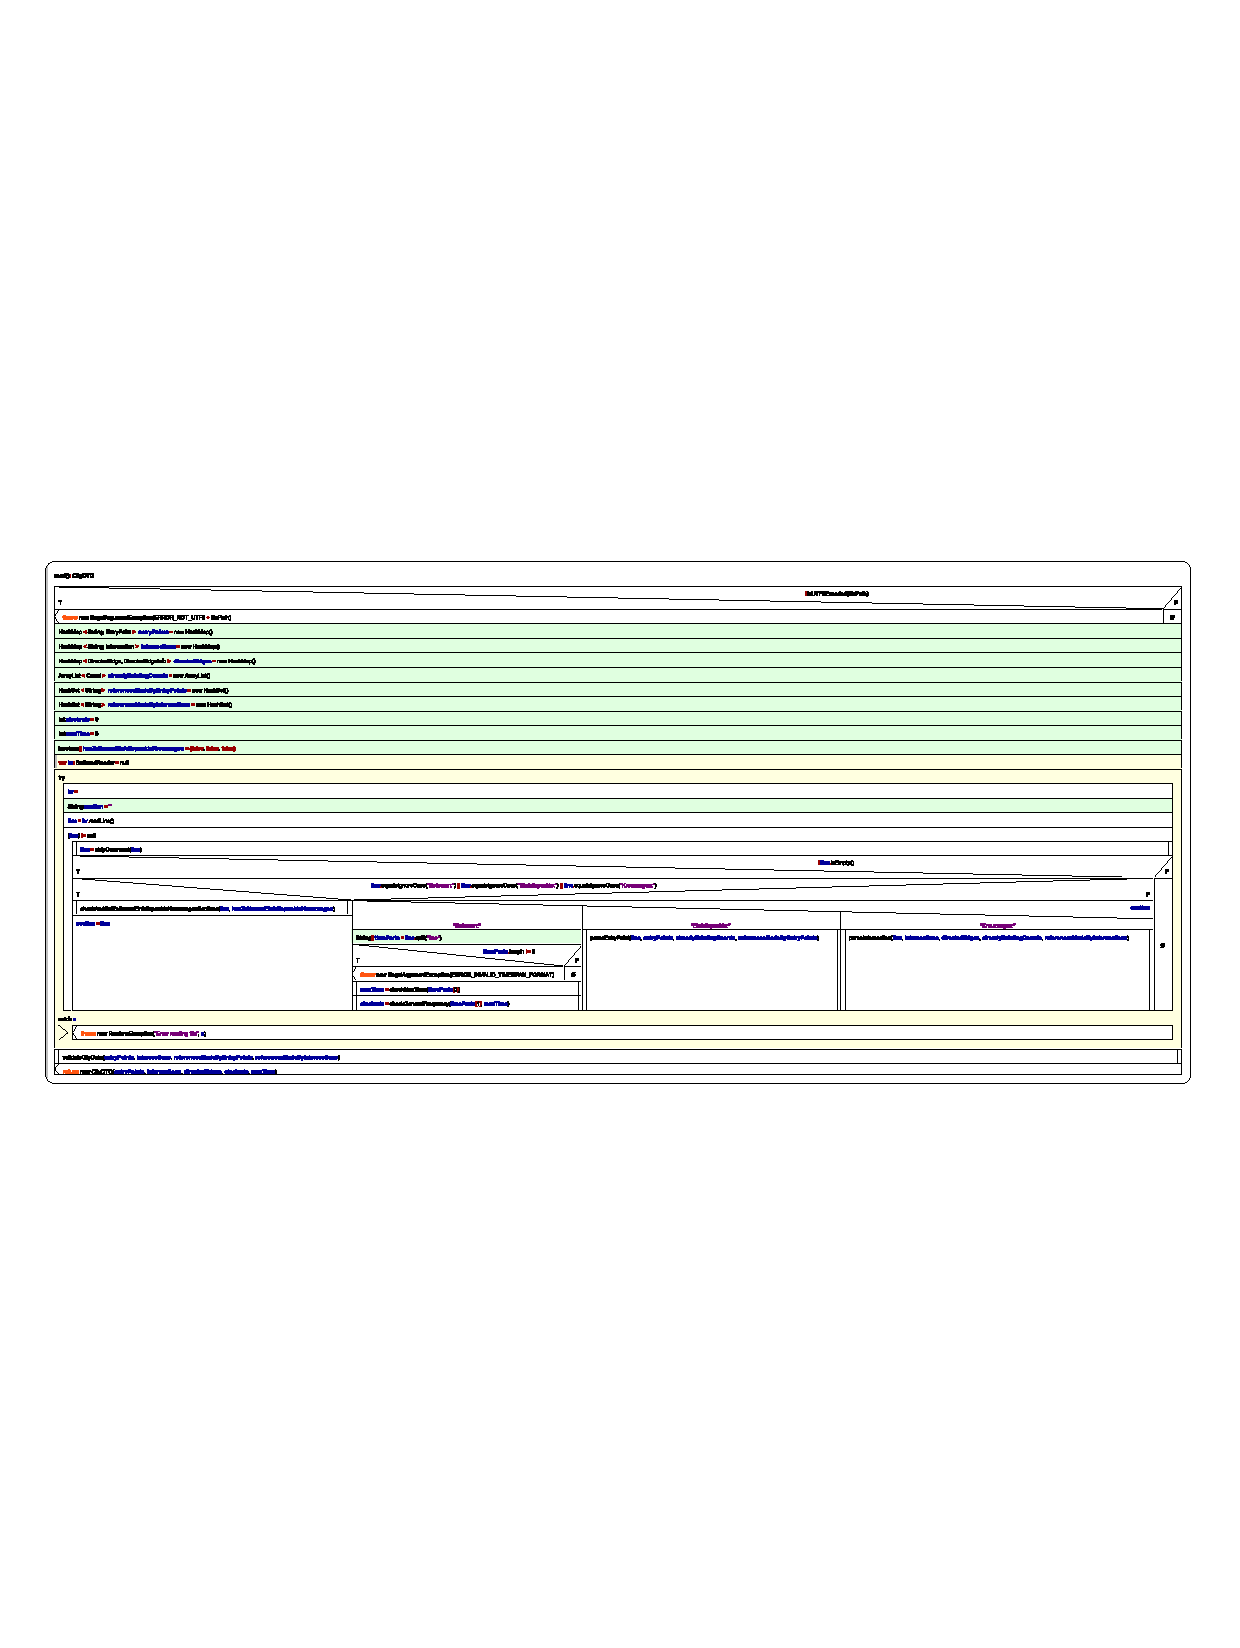
\includegraphics[width=1.5\textwidth]{nassis/TextFileReader/read-0.pdf}}
\end{figure}
\clearpage
\section{Datenhaltung}


Die Datenhaltung der Simulation erfolgt über Klassen, welche die Elemente des Verkehrsnetzes sowie den Zustand der Simulation abbilden.

\begin{itemize}
  \item \textbf{\texttt{CityDTO}}\\
  Dieses Datenübertragungsobjekt (\emph{Data Transfer Object}) bündelt alle zur Initialisierung der Simulation notwendigen Informationen:
  \begin{itemize}
    \item \texttt{entryPoints} -- Einfallspunkte als Map von Namen auf \texttt{EntryPoint}-Objekte,
    \item \texttt{intersections} -- Kreuzungen als Map von Namen auf \texttt{Intersection}-Objekte,
    \item \texttt{directedEdges} -- Gerichtete Kanten zwischen Knoten, jeweils mit zugehörigem \texttt{DirectedEdgeInfo},
    \item \texttt{clockRate} und \texttt{maxTime} -- Zeitparameter der Simulation.
  \end{itemize}

  \item \textbf{\texttt{Coord}}\\
  Diese Klasse repräsentiert zweidimensionale Koordinaten.
  Sie enthält Methoden zur Vektoroperation (Addition, Subtraktion, Normalisierung, Skalierung) sowie zur Berechnung von Distanzen.
  Die Koordinaten dienen als Grundlage für Bewegungsrichtungen und Standortspeicherungen.

  \item \textbf{\texttt{DirectedEdge}}\\
  Modelliert eine gerichtete Verbindung zwischen zwei Punkten im Verkehrsnetz.
  Zwei Felder (\texttt{from}, \texttt{to}) beschreiben die Richtung. \texttt{equals()} und \texttt{hashCode()} sind überschrieben, um die Kante als Schlüssel in HashMaps verwenden zu können.

  \item \textbf{\texttt{DirectedEdgeInfo}}\\
  Diese Klasse hält statistische Informationen zu jeder Kante:
  \begin{itemize}
    \item \texttt{totalCount} -- Gesamtanzahl aller Fahrzeuge, die die Kante jemals befahren haben,
    \item \texttt{currentNum} -- Aktuelle Anzahl an Fahrzeugen auf der Kante,
    \item \texttt{maxNum} -- Maximalanzahl an Fahrzeugen, die gleichzeitig auf der Kante waren.
  \end{itemize}
  Methoden wie \texttt{increment()}, \texttt{decrement()} und \texttt{updateMaxNum()} aktualisieren die Werte während der Simulation.

  \item \textbf{\texttt{EntryPoint}}\\
  Stellt einen Punkt dar,
  an dem Fahrzeuge ins Netz eintreten.
  Neben der Position (\texttt{coord}) enthält das Objekt den Namen der Zielkreuzung sowie die Erzeugungsfrequenz (\texttt{freq}) neuer Fahrzeuge.

  \item \textbf{\texttt{Intersection}}\\
  Repräsentiert eine Kreuzung im Verkehrsnetz.
  Enthält eine Position und ein \texttt{NamesAndProbabilities}-Objekt,
  das die möglichen Ausfahrten mit Wahrscheinlichkeiten beschreibt.
  Methoden wie \texttt{getNewDestinationByProbability()} wählen anhand eines Zufallswerts ein neues Ziel aus.

  \item \textbf{\texttt{NamesAndProbabilities}}\\
  Eine einfache Container-Klasse für Kreuzungsverbindungen. Sie enthält zwei Arrays:
  \begin{itemize}
    \item \texttt{names} -- Zielknoten,
    \item \texttt{probabilities} -- Normalisierte Übergangswahrscheinlichkeiten.
  \end{itemize}
  Diese Struktur erleichtert die Auswahl des nächsten Ziels für Fahrzeuge an Kreuzungen.
  Denn die Wahrscheinlichkeiten müssen an jeder Kreuzung normalisiert werden, da Fahrzeuge nicht in die Richtung zurückfahren können, aus der sie gekommen sind.

  \item \textbf{\texttt{Vehicle}}\\
  Diese Klasse beschreibt den Zustand eines einzelnen Fahrzeugs.
  Sie enthält Informationen zur aktuellen Position, Bewegungsrichtung, Geschwindigkeit sowie zur Herkunft und dem Ziel.
  Die \texttt{clone()}-Methode erlaubt die Erstellung tiefer Kopien zur Historisierung der Fahrzeugbewegungen.
  Geschwindigkeit und Richtung werden kontinuierlich in der simulate() Methode der City Klasse berechnet.
\end{itemize}

Das folgende Diagramm zeigt die Struktur der Datenhaltungsklassen und deren Beziehungen zueinander.
\begin{figure}[h!]
    \centering
    %\caption{Klassenstruktur der Simulation}
    \makebox[\textwidth][c]{\includegraphics[width=1.3\textwidth]{umlClassDiagrams/dataHolders.png}}
\end{figure}

\clearpage

\section{Simulation}

Die Klasse City übernimmt die zentrale Steuerung der Simulation und verwaltet alle strukturellen Elemente des Straßennetzes.
Dazu zählen Einfallspunkte (EntryPoint), Kreuzungen (Intersection) sowie gerichtete Straßenverbindungen (DirectedEdge).
Neben diesen Strukturinformationen enthält die Klasse eine Liste aktuell aktiver Fahrzeuge sowie eine Historie aller Fahrzeugzustände,
die zu Analysezwecken gespeichert wird.

Der Simulationsablauf wird durch die Methode simulate() umgesetzt,
die für jeden Zeitschritt folgende Operationen durchführt:

Bewegung der Fahrzeuge: Die Methode updateVehicles() iteriert über alle aktiven Fahrzeuge und aktualisiert deren Position.
Wenn ein Fahrzeug sein Ziel erreicht hat,
wird es entweder entfernt (bei Ankunft an einem Einfallspunkt) oder ihm wird anhand der Wahrscheinlichkeiten an der aktuellen Kreuzung ein neues Ziel zugewiesen.
An jeder Kreuzung werden die relativen Wahrscheinlichkeiten neu berechnet, da Fahrzeuge nicht in die Richtung zurückfahren dürfen, aus der sie gekommen sind.
Die Neuberechnung der Wahrscheinlichkeiten erfolgt durch Normalisierung. Dabei wird die Wahrscheinlichkeit für ein Wenden ignoriert,
und alle verbleibenden Wahrscheinlichkeiten werden durch die Summe der übrigen Wahrscheinlichkeiten (alle außer die Wendewahrscheinlichkeit) geteilt.

Zur Auswahl der Straße, auf die mit proportionaler Wahrscheinlichkeit abgebogen werden soll, wird der „Roulette-Wheel-Selection“-Algorithmus verwendet. 
Dabei wird zunächst eine gleichverteilte Zufallszahl zwischen 0 und 1 generiert. Anschließend wird überprüft, ob der Wert der ersten Wahrscheinlichkeit größer oder gleich der erzeugten Zufallszahl ist. 
Falls dies nicht der Fall ist, wird die nächste Wahrscheinlichkeit aufaddiert und der Vergleich wiederholt, bis die kumulierte Wahrscheinlichkeit größer oder gleich der Zufallszahl ist. 
Der Index der zuletzt hinzugefügten Wahrscheinlichkeit entspricht der mit proportionaler Wahrscheinlichkeit ausgewählten Straße.

Die Bewegung wird unter Beibehaltung der Restgeschwindigkeit auf die neue Verbindung fortgesetzt.

Fahrzeugerzeugung: Zu festgelegten Zeitintervallen (abhängig vom Taktwert des jeweiligen Einfallspunkts) wird ein neues Fahrzeug erzeugt.
Die Methode createNewVehicle() initialisiert dessen Position, Ziel, Bewegungsrichtung und Geschwindigkeit.
Die Geschwindigkeit wird normalverteilt mit einem Erwartungswert von 45 km/h und einer Standardabweichung von 10 km/h erzeugt.
Hierzu wird eine standardnormalverteilte Zufallsvariable (\(N(0,1)\)) generiert, mit der Standardabweichung multipliziert und anschließend zum Erwartungswert addiert.
Die Geschwindigkeit wird zuvor in die Einheit von 100 Metern umgerechnet.
Jede Zufallszahl wird mithilfe eines Pseudozufallsgenerators (\texttt{java.util.Random}) erzeugt.
Außerdem wird die zugehörige Kante im Verkehrsnetz bei Fahrzeugeintritt aktualisiert.

Statistikerhebung: Nach jedem Zeitschritt wird für jede Kante im Netz die aktuelle Anzahl an Fahrzeugen geprüft und ggf. ein neuer Maximalwert gespeichert (updateDirectedEdgesMaxima()).

Aufzeichnung des Systemzustands: In Abständen, die durch den clockRate bestimmt werden,
wird der Zustand aller Fahrzeuge als tiefe Kopie in einer Historie (vehicleHistory) gespeichert.
Diese erlaubt eine spätere zeitbasierte Rekonstruktion der Fahrzeugbewegungen.

Das folgende Klassen-Diagramm zeigt die Struktur der City-Klasse und die nachfolgenden Nassi-Shneiderman-Diagramme verdeutlichen die oben beschriebene Funktionsweise.

\begin{figure}[h!]
    \centering
    \makebox[\textwidth][c]{\includegraphics[width=1.3\textwidth]{umlClassDiagrams/cityBasicUmlClassDiagram.png}}
\end{figure}

\begin{figure}[h!]
    \centering
    \makebox[\textwidth][c]{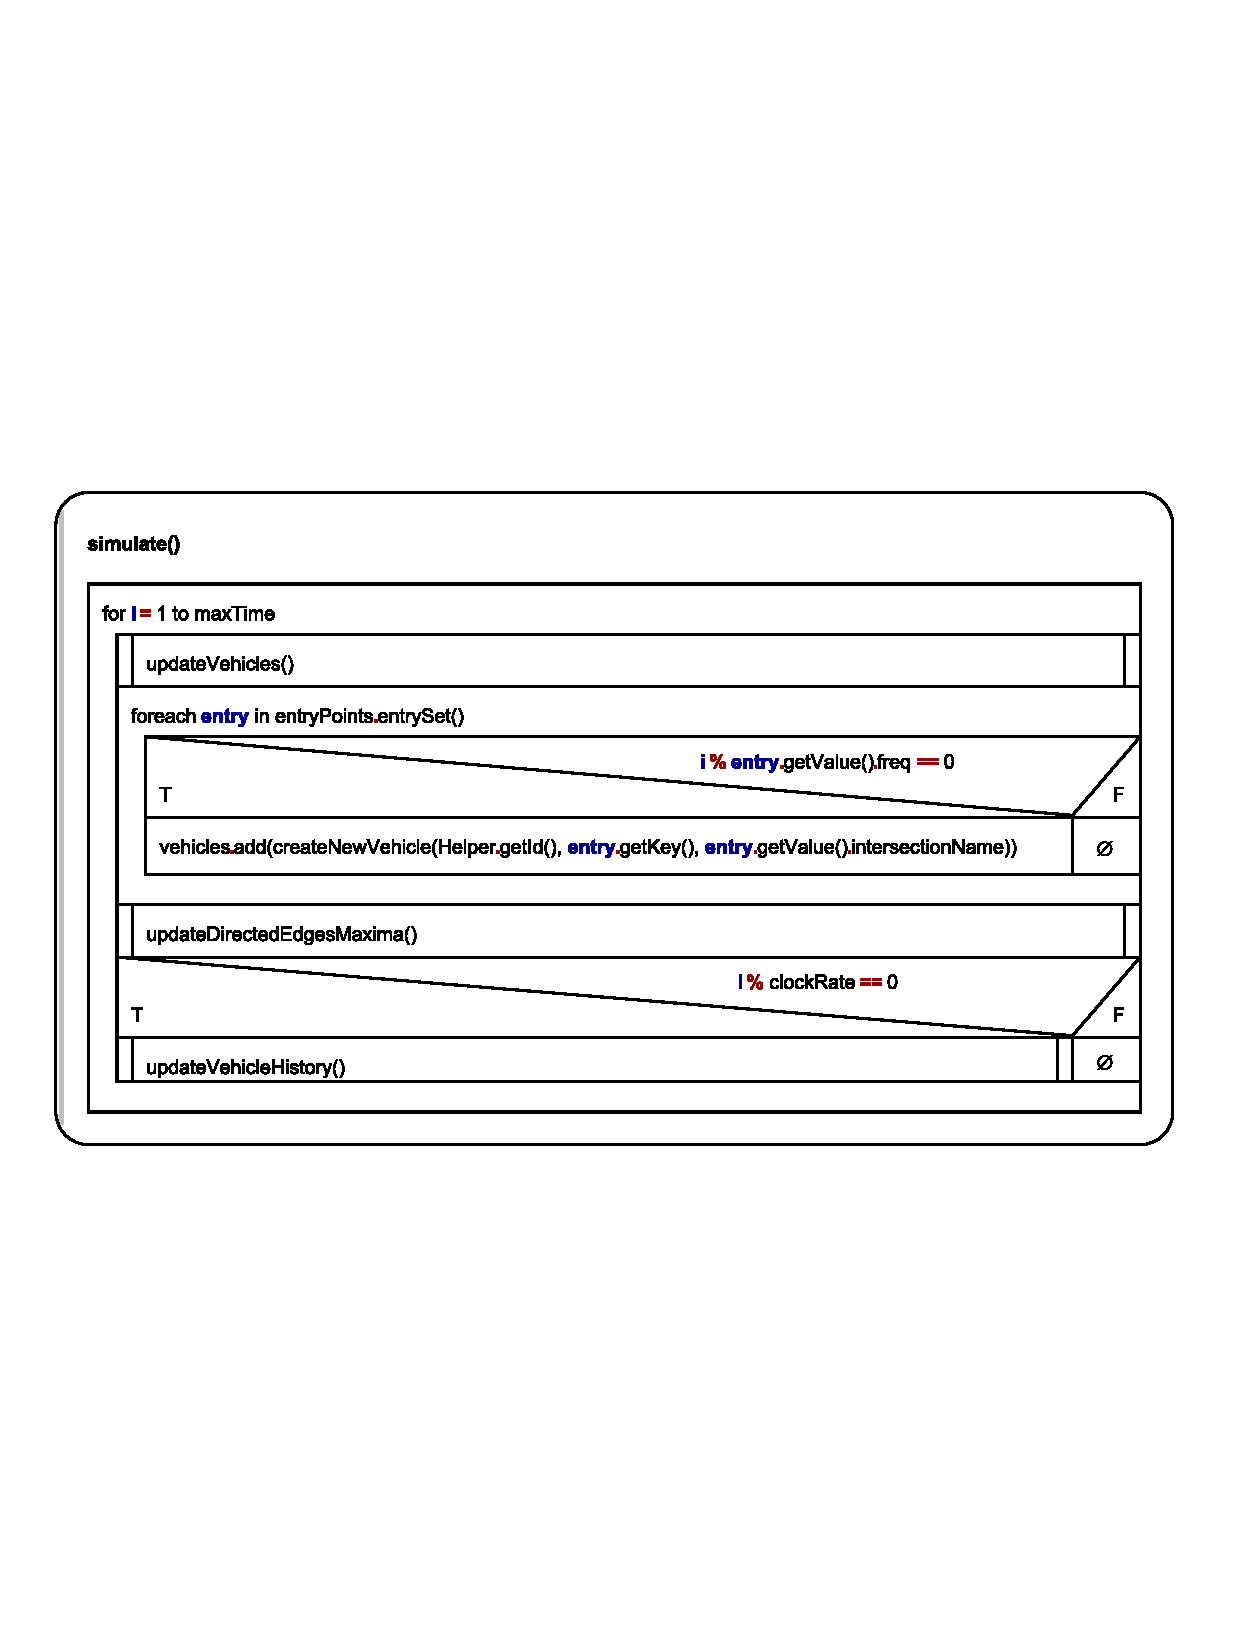
\includegraphics[width=1.3\textwidth]{nassis/City/simulate-0.pdf}}
\end{figure}

\begin{figure}[h!]
    \centering
    \makebox[\textwidth][c]{\includegraphics[width=1.3\textwidth]{nassis/City/updateVehiclesAndCreateNewVehiclesCombined.pdf}}
\end{figure}


\begin{figure}[h!]
    \centering
    \makebox[\textwidth][c]{\includegraphics[width=1.3\textwidth]{nassis/City/updateMaximaAndHistory.pdf}}
\end{figure}

\FloatBarrier
Darüber hinaus stellt die Klasse Funktionen zur Verfügung,
um alle gerichteten Kanten alphabetisch sortiert auszulesen (getAlphabeticallySortedDirectedEdges()),
was für die strukturierte Ausgabe der Ergebnisse genutzt wird.

\cleardoublepage

\section{Ausgabe}

Nach Abschluss der Simulation werden die Ergebnisse in drei getrennte Ausgabedateien geschrieben.
Die hierfür verantwortlichen Klassen befinden sich im Output Verzeichnis des trafficsimulation packages.

\begin{itemize}
  \item \textbf{\texttt{Plan.txt} (Klasse \texttt{PlanWriter})} \\
  Diese Datei enthält alle gerichteten Straßenverbindungen als Koordinatenpaare:
  \begin{center}
    \texttt{x1 y1 x2 y2}
  \end{center}
  wobei \texttt{x1 y1} die Start- und \texttt{x2 y2} die Zielposition einer Kante angeben. Die Ausgabe erfolgt alphabetisch sortiert nach Start- und Zielnamen.

  \FloatBarrier
    \vspace{-2cm} 
\begin{figure}[h!]
    \vspace{-2cm} 
    \centering
    \makebox[\textwidth][c]{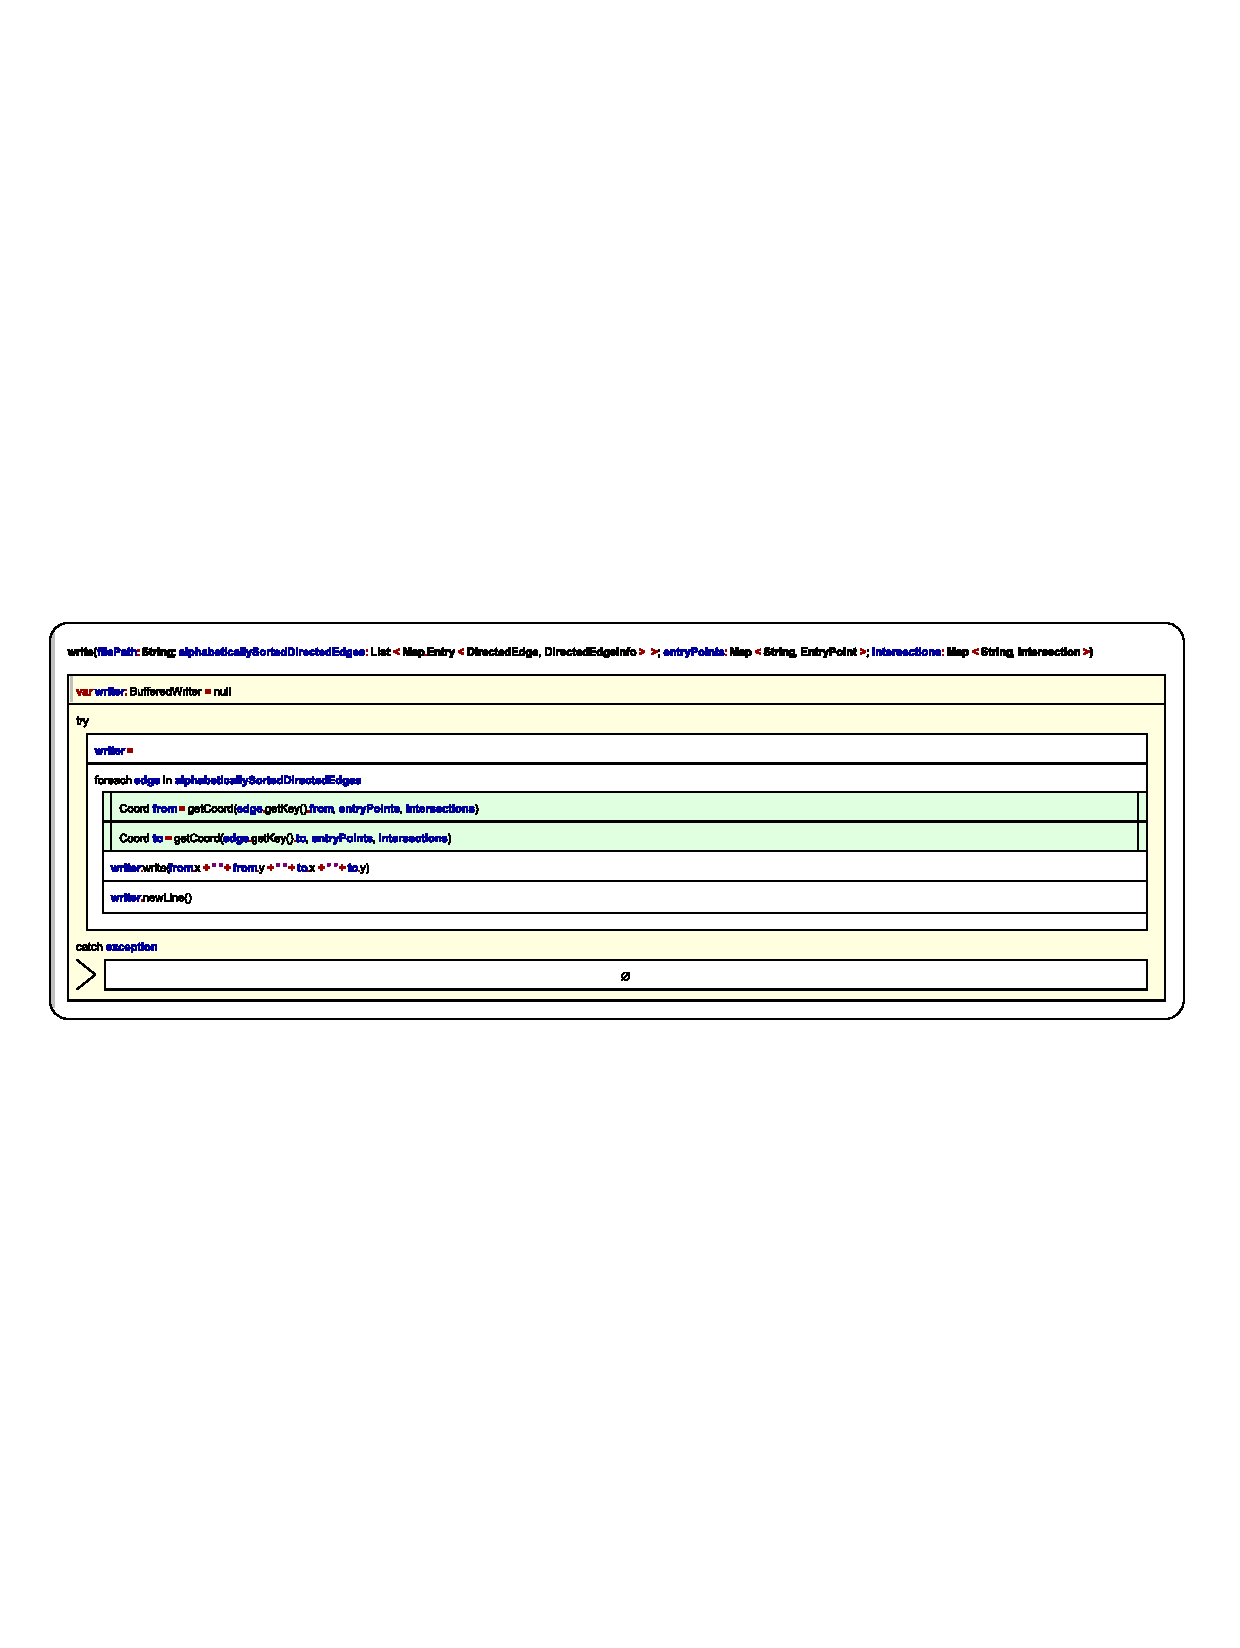
\includegraphics[width=1.05\textwidth]{nassis/OutputWriters/write-4.pdf}}
\end{figure}

\clearpage

  \item \textbf{\texttt{Statistik.txt} (Klasse \texttt{StatisticWriter})} \\
  Für jede Kante werden zwei Werte normiert auf 100 Meter Straßenlänge berechnet und ausgegeben:
  \begin{itemize}
    \item \textbf{Gesamtanzahl Fahrzeuge:} Wie viele Fahrzeuge die Kante insgesamt passiert haben.
    \item \textbf{Maximale Anzahl Fahrzeuge:} Die maximale Anzahl gleichzeitig auf der Kante befindlicher Fahrzeuge während der Simulation.
  \end{itemize}
  Beide Werte werden berechnet, indem die Rohwerte durch die euklidische Länge der jeweiligen Kante geteilt werden, wobei die Berechnung auf 100 Meter normiert ist.
  Die Ausgabe erfolgt ebenfalls alphabetisch sortiert nach Start- und Zielnamen.

  \FloatBarrier
      \vspace{-2cm} 
\begin{figure}[h!]
        \vspace{-2cm} 
    \centering
    \makebox[\textwidth][c]{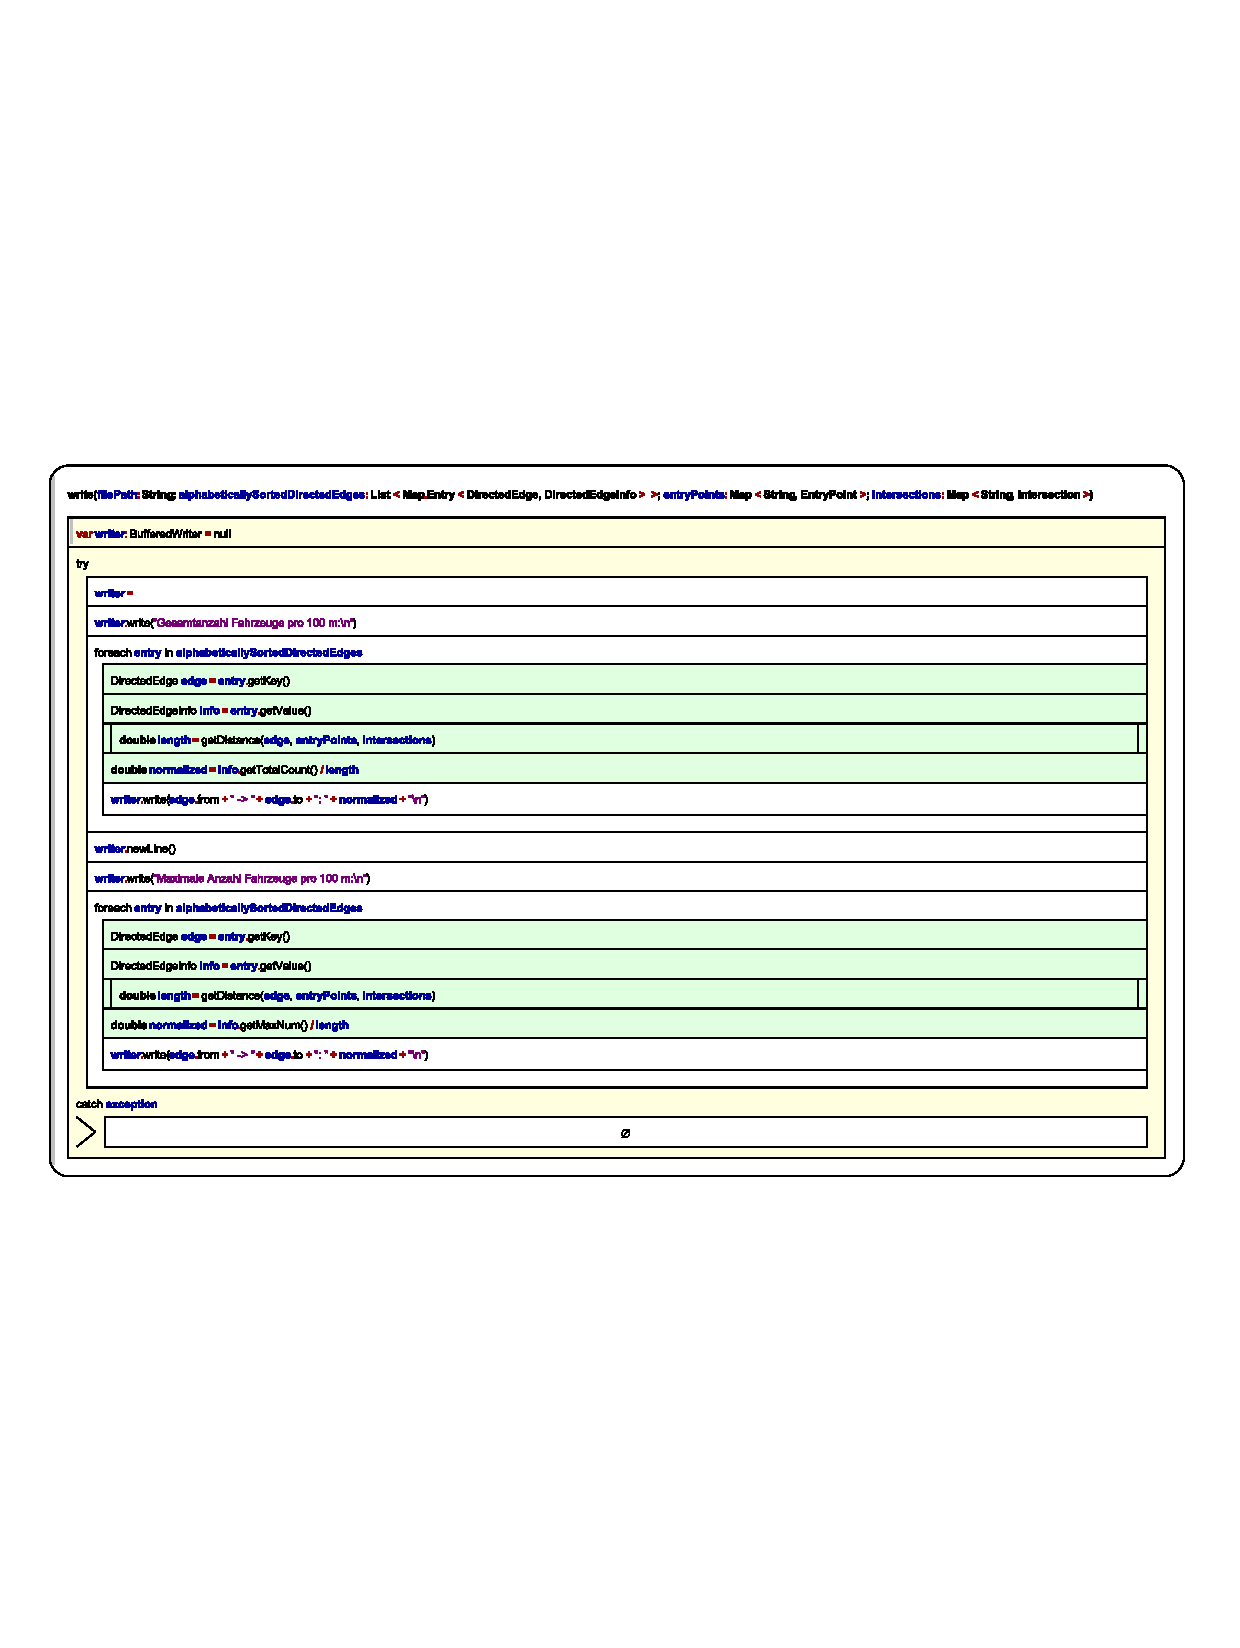
\includegraphics[width=1.05\textwidth]{nassis/OutputWriters/writeStats.pdf}}
\end{figure}

\clearpage

  \item \textbf{\texttt{Fahrzeuge.txt} (Klasse \texttt{VehicleWriter})} \\
  Diese Datei protokolliert die Positionen aller Fahrzeuge zu bestimmten Zeitpunkten der Simulation (gesteuert durch den Parameter \texttt{clockRate}). Jeder Zeitstempel ist mit \texttt{*** t = <Sekunden>} markiert. Darunter folgen Zeilen mit:
  \begin{center}
    \texttt{<x\_pos> <y\_pos> <x\_ziel> <y\_ziel> <ID>}
  \end{center}
  Dadurch kann der zeitliche Verlauf der Fahrzeugbewegungen nachvollzogen werden. Die Daten stammen aus der \texttt{vehicleHistory}.
\end{itemize}

\FloatBarrier
        \vspace{-2cm} 
\begin{figure}[h!]
            \vspace{-2cm} 
    \centering
    \makebox[\textwidth][c]{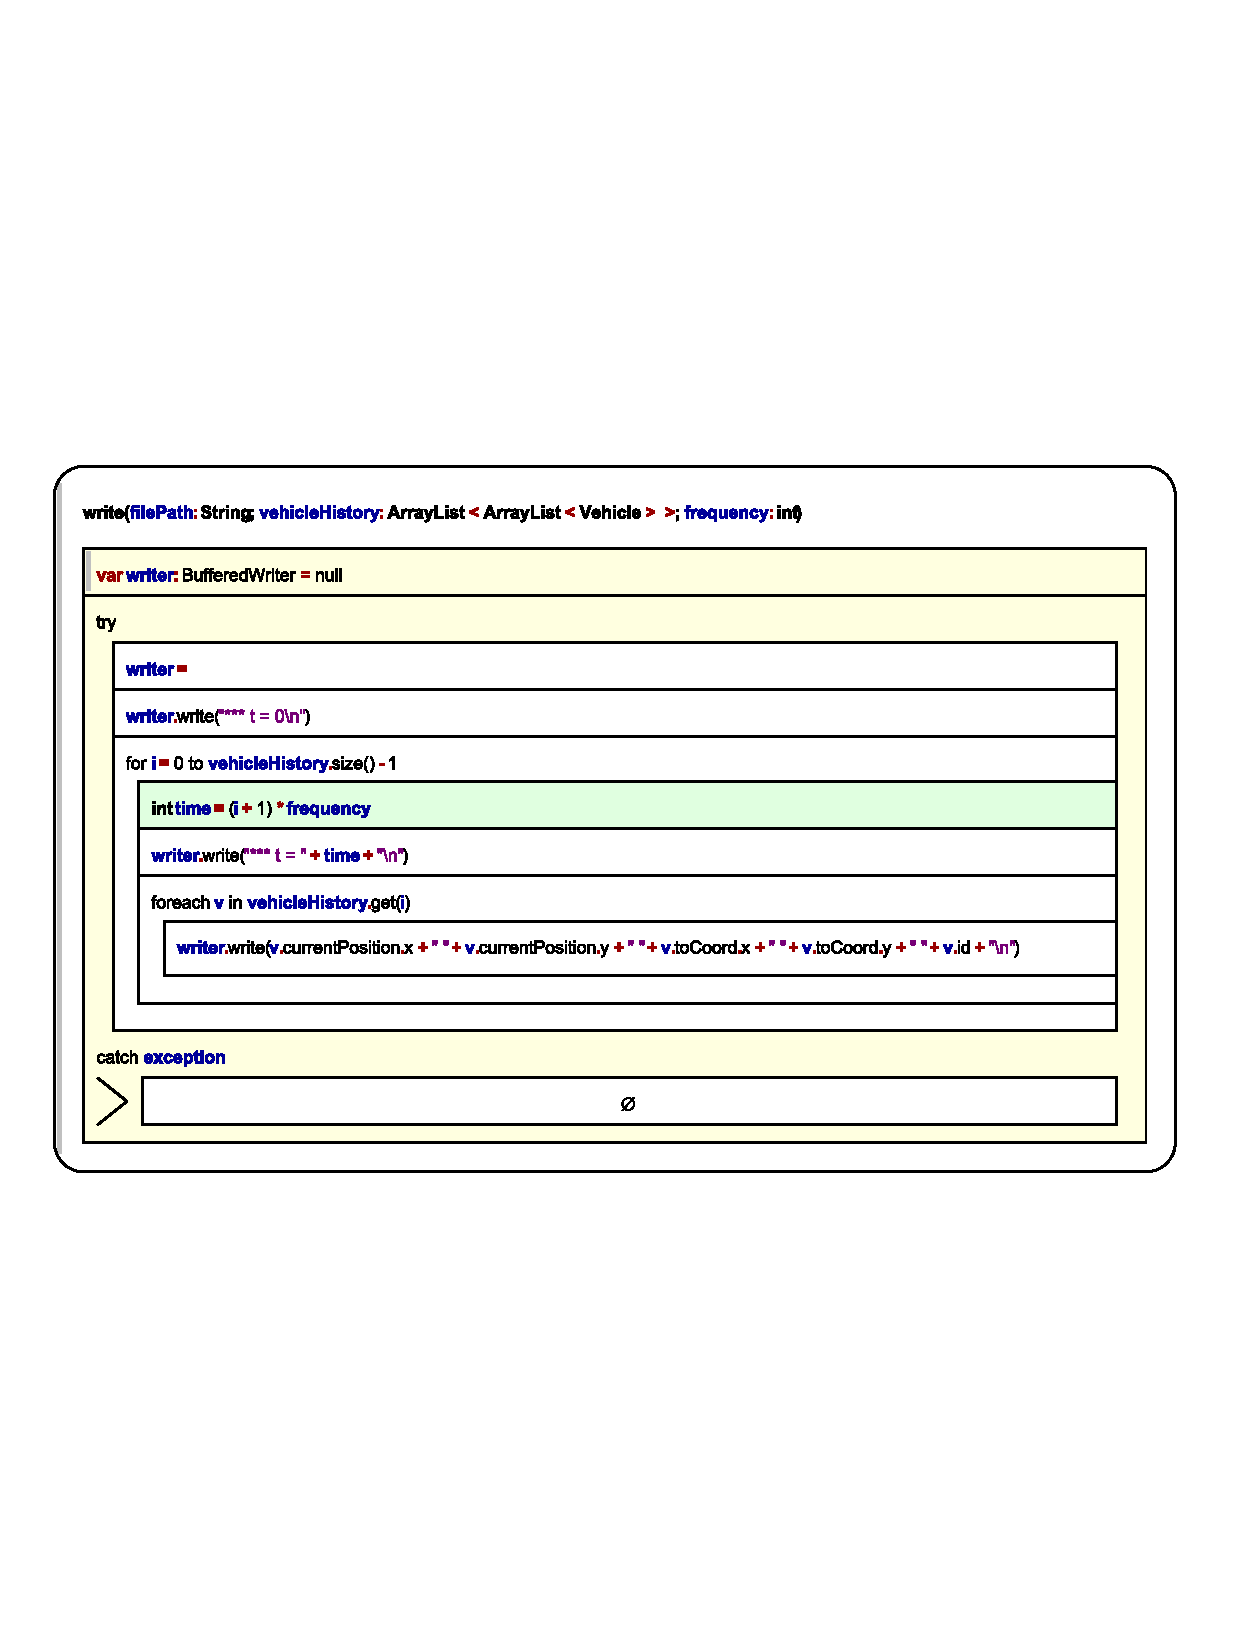
\includegraphics[width=1.05\textwidth]{nassis/OutputWriters/writeVehicles.pdf}}
\end{figure}
\FloatBarrier
\vspace{-2cm}
\begin{figure}[h!]
    \vspace{-2cm}
    \centering
    \caption{Klassenstruktur der Ausgabeklassen}
    \makebox[\textwidth][c]{\includegraphics[width=1.05\textwidth]{umlClassDiagrams/outputUml.png}}
\end{figure}


\clearpage

\section{Gesamtablauf}

\begin{enumerate}
  \item \textbf{Programmstart (\texttt{Main.main})}
  \begin{itemize}
    \item Prüfung, ob ein gültiger Dateipfad als Argument übergeben wurde.
    \item Instanziierung eines \texttt{Reader}-Objekts vom Typ \texttt{TextFileReader}.
  \end{itemize}

  \item \textbf{Einlesen der Stadtstruktur (\texttt{reader.read()})}
  \begin{itemize}
    \item Datei wird zeilenweise eingelesen und in Abschnitte gegliedert:
    \begin{itemize}
      \item \texttt{Zeitraum:} Einlesen von \texttt{maxTime} und \texttt{clockRate}.
      \item \texttt{Einfallspunkte:} Aufbau einer Map von Namen auf \texttt{EntryPoint}-Objekte.
      \item \texttt{Kreuzungen:} Aufbau einer Map von Namen auf \texttt{Intersection}-Objekte sowie gerichteter Kanten mit zugehörigem \texttt{DirectedEdgeInfo}.
    \end{itemize}
    \item Durchführung mehrerer Validierungen (z.\,B. doppelte Namen, unerlaubte Referenzen, Mindestabstand von Koordinaten).
    \item Rückgabe eines \texttt{CityDTO}-Objekts.
  \end{itemize}

  \item \textbf{Initialisierung der Simulation (\texttt{new City(CityDTO)})}
  \begin{itemize}
    \item Übernahme aller Eingabedaten in das \texttt{City}-Objekt.
  \end{itemize}

  \item \textbf{Simulationsablauf (\texttt{city.simulate()})}
  \begin{itemize}
    \item Für jede Zeiteinheit $t$ von $1$ bis \texttt{maxTime}:
    \begin{itemize}
      \item \texttt{updateVehicles()}: Bewegung aller Fahrzeuge entlang ihrer aktuellen Kante. Bei Zielerreichung Auswahl eines neuen Ziels oder Entfernen des Fahrzeugs.
      \item Fahrzeugerzeugung an jedem Einfallspunkt, sofern $t \mod \texttt{freq} = 0$.
      \item \texttt{updateDirectedEdgesMaxima()}: Aktualisierung der Maximalwerte pro Kante.
      \item Speicherung eines Snapshots der Fahrzeugzustände in \texttt{vehicleHistory}, wenn $t \mod \texttt{clockRate} = 0$.
    \end{itemize}
  \end{itemize}

  \item \textbf{Erzeugung der Ausgabedateien}
  \begin{itemize}
    \item \texttt{PlanWriter.write}: Ausgabe aller Straßenverbindungen (Koordinatenpaare) in \texttt{Plan.txt}.
    \item \texttt{StatisticWriter.write}: Ausgabe von Nutzungsstatistiken (gesamt / maximal pro 100\,m) in \texttt{Statistik.txt}.
    \item \texttt{VehicleWriter.write}: Ausgabe aller Fahrzeugpositionen zu gespeicherten Zeitpunkten in \texttt{Fahrzeuge.txt}.
  \end{itemize}
\end{enumerate}

\begin{figure}[h!]
    \centering
    \caption{Hauptablauf der Simulation}
    \makebox[\textwidth][c]{\includegraphics[width=1.3\textwidth]{umlClassDiagrams/MainSequenceDiagram.png}}
\end{figure}





\chapter{Abweichungen vom ersten Entwurf}
Bei der Implementierung wurden einige Abweichungen vom ersten Entwurf vom Montag, den 12.05.2025, vorgenommen.
So wurde eine \texttt{CityDTO}-Datentransferklasse geschrieben, die verwendet wird, um ein \texttt{City}-Objekt zu instanziieren.
Dies ist angenehmer als die Nutzung eines Konstruktors mit fünf Eingabeparametern und erfordert keine Implementierung von
fünf \texttt{get}-Methoden in der \texttt{TextFileReader}-Klasse.

Die Klasse \texttt{TrafficNode}, die eine Kreuzung darstellen sollte, erhielt den passenderen Namen \texttt{Intersection}.
Es wurde eine Helper-Klasse mit einer statischen \texttt{getId()}-Methode implementiert, um die Fahrzeug-IDs zu generieren.

Im UML-Klassendiagramm der \texttt{Vehicle}-Klasse wurde das Attribut \texttt{double velocity} (für Geschwindigkeit) vergessen (existiert in der finalen Implementierung).
Anfangs wurde nicht spezifiziert, dass die Ausgabe in den Dateien \texttt{Plan.txt} und \texttt{Statistik.txt} nach alphabetisch sortierten Eingabeortsnamen erfolgen soll.
Deswegen wurde die Methode \texttt{getAlphabeticallySortedDirectedEdges()} geschrieben.

Die Methode \texttt{updateVehicle()} erhält einen \texttt{Iterator<Vehicle>} anstelle eines einzelnen \texttt{Vehicle}-Objekts, um ein sicheres Entfernen zu gewährleisten,
z. B. wenn ein Fahrzeug den Stadtplan über einen Einfallspunkt verlässt, während die Fahrzeugliste iteriert wird.

Die Methode \texttt{considerVehiclesThatAreStillDriving()}, die ursprünglich dazu gedacht war, Fahrzeuge,
die nach Ende der Simulationszeit noch unterwegs sind, in die Statistik aufzunehmen,
erwies sich als unnötig, da die Statistikberechnung Fahrzeuge bereits als den Abschnitt gefahren zählt,
sobald sie auf den jeweiligen Abschnitt auffahren.

Eine Reihe von \texttt{get}-Methoden wurde hinzugefügt, um den Outputwritern \\
(z. B. \texttt{PlanWriter}) die benötigten Informationen wie die \texttt{directedEdges} bereitzustellen.

Einige Anforderungen vom Montag wurden revidiert. So wurde ursprünglich festgelegt, dass jede Kreuzung mindestens drei Abbiegepunkte haben soll.
Da dies die Eingabe des „IHK-Beispiels Tunneldorf mit Umfahrung über I“ ungültig machen würde, wurde davon abgewichen,
sodass jede Kreuzung nun nur mindestens zwei verbindende Straßen haben muss.
In der Anfangsspezifikation wurde fälschlicherweise angenommen, dass die relativen Wahrscheinlichkeiten einer Kreuzung in
Prozent angegeben sind und sich zu 100 aufaddieren. Dies wurde geändert, sodass alle relativen Wahrscheinlichkeiten intern normiert werden.





\chapter{Tests}

Das Verifizieren, ob die Ausgabedateien korrekt sind,
lässt sich aufgrund der zufälligen Natur der Simulation und der fehlenden Vergleichsmöglichkeiten mit erwartetem Output
nur visuell über das PLot.py Skript.

Die Normalfälle von der IHK Website getestet und visuell als passend empfunden.
Ein Fokus wurde auf das Testen von Fehler und Grenzfällen bei der Einlese gelegt.

Hierfür wurde ein Ordner namens badInputTests erstellt und

\section{Ausführen der Tests}

\subsection{BadInputTestRunner}

Bei der Arbeit an dem TextFileReader wurde mehrfach refactored und die Bedingungsprüfungen wurden nacheinander implementiert und nach jeder Bedingung geprüft, 
ob frühere Fehlerfälle immer noch die erwartete Ausgabe liefern. 
Um diesen Prozess zu automatisieren, wurde das \texttt{BadInputTestRunner}-Testprogramm für Regressionstests geschrieben.

Der Quellcode ist die gleichnamige Java-Datei im \texttt{tests}-Ordner, ebenfalls im \\
\texttt{trafficsimulation}-Package. 
Das Programm führt die folgenden Schritte aus:

\begin{itemize}
    \item \textbf{Verzeichnisprüfung:} Es wird geprüft, ob das Verzeichnis \texttt{badInputTests} existiert und Eingabedateien enthält.
    \item \textbf{Definition der Testfälle:} Für jede fehlerhafte Eingabedatei wird die erwartete Fehlermeldung definiert. Beispiele für Fehler sind:
    \begin{itemize}
        \item Fehlende Einfallspunkte (\texttt{ERROR\_NO\_ENTRY\_POINTS}),
        \item Ungültige Koordinaten (\texttt{ERROR\_INVALID\_COORDINATE\_COMPONENT})
    \end{itemize}
    \item \textbf{Testausführung:} Jede Eingabedatei wird mit dem \texttt{TextFileReader} eingelesen. Falls die Datei fehlerhaft ist, wird eine Ausnahme ausgelöst.
    \item \textbf{Ergebnisprüfung:} Die tatsächliche Fehlermeldung wird mit der erwarteten Fehlermeldung verglichen. Stimmen sie überein, gilt der Test als bestanden.
    \item \textbf{Endergebnis:} Am Ende wird eine Übersicht ausgegeben, ob alle Tests bestanden wurden oder ob Fehler aufgetreten sind.
\end{itemize}


Zum Testen des Programms steht je ein Skript für Windows und Linux/macOS zur Verfügung. Unter Windows wird das Skript \texttt{test\_run.bat} verwendet.
Es führt die Datei \texttt{MyProgram.jar} für jede Datei im Ordner \texttt{input\_files} einzeln aus und übergibt sie als Argument an das Programm.

Zur Ausführung müssen alle Eingabedateien im Verzeichnis \texttt{input\_files} liegen und sich die \texttt{.jar}-Datei im gleichen Ordner wie das Skript befinden.
Das Skript kann entweder per Doppelklick oder über die Eingabeaufforderung mit \texttt{test\_run.bat} gestartet werden.

Für Linux oder macOS wird das Bash-Skript \texttt{test\_run.sh} genutzt. Auch hier wird die \texttt{MyProgram.jar} für jede Datei im Ordner \texttt{input\_files} aufgerufen.

Vor dem ersten Ausführen muss dem Skript Ausführungsrecht gegeben werden, z.\,B.\ durch den Befehl \texttt{chmod +x test\_run.sh}. Danach kann es mit \texttt{./test\_run.sh} ausgeführt werden.
Alternativ kann das Skript auch ohne Ausführungsrecht mit \texttt{bash test\_run.sh} gestartet werden.

\chapter{Erweiterbarkeit}

Eine vorstellbare weitere Anforderung wäre, 
dass Fahrzeuge nicht überholen können, sondern einen Mindestabstand zum vorausfahrenden Fahrzeug einhalten müssen.
Diese zusätzliche Anforderung ließe sich durch Anpassen der DirectedEdgeInfo Klasse und der updateVehicle Methode erreichen.
Die Fahrzeuge würden nicht mehr zentral in der vehicles Liste gespeichert werden, sondern in der DirectedEdgeInfo Klasse in einer
Queue Struktur. Neue Fahrzeuge auf der Straße würden ans Ende der Queue eingefügt werden und Fahrzeuge, die die Straße verlassen, 
würden, würden am Anfang der Queue entfernt werden.
Beim Aktualisieren der Fahrzeuge in der simulate() Methode würde über die DirectedEdgeInfos in der directedEdges HashMap iteriert werden
und die Position des Fahrzeugs, welches am nächsten am Verlassen der Straße ist, würde als erstes aktualisiert werden, also das Fahrzeug, welches am Anfang der 
Straßenqueue ist. Bei dem ersten aktualisierten Fahrzeug würde berechnet werden, wo ein Fahrzeug, welches den Minimalabstand zu dem Fahrzeug am Anfang der Queue einhält, wäre und diese Position wird an
das zweite Fahrzeug weitergegeben. Nun wird die Position des zweiten Fahrzeuges so angepasst, dass dieses entweder normal weiterfährt, wenn es nicht den Minimalabstand unterschreiten würde oder,
wenn es den Minimalabstand unterschreiten würde die Position auf die übergebene zuvor berechnete Position gesetzt.
Am Ende aller Iterationen aller DirectedEdges, werden die Positionen der Fahrzeuge neu berechnet, welche Straßen an Kreuzungen gewechselt haben.

Wenn der Verkehrsfluss an Kreuzungen über Ampeln geregelt werden würde, würde die Position von Fahrzeugen,
die eine Straße an einer Kreuzung wechseln würde um die Anzahl an Takten, wie lange die Ampel gehen würde gestoppt, bevor diese weiterfahren dürfen.

Beim Hinzufügen von Kreisverkehren wäre eine ähnliche Logik anwendbar. Ein Fahrzeug würde für die Taktlänge eines im Stadtplan durch ein extra Zeichen angegebenen Kreisverkehr
an der Kreuzung verweilen, bevor diese weiterfährt.

Für das Implementieren einer Rechts vor Links Überprüfung müsste man für jedes Fahrzeug, welches eine Kreuzung passieren würde erstmal prüfen,
welche Straßen rechts sind. Dafür würde man die xy Komponenten des Anfangs End Vektors der gerade gefahrenen Straße tauschen und danach die y Komponente negieren,
um den links orthogonalen Vektor zu dem gerade gefahrenen Straßenvektor zu erhalten. Nun findet man alle directedEdges bei denen to der Kreuzung entspricht an der abgebogen werden soll.
Von diesen sind die Straßen rechts, bei denen das Skalarprodukt des links orthogonalen Vektor mit dem Anfangs End Vektor der potentiellen rechts Straße größer 0 ist.

Jetzt muss berechnet werden, ob mehrere Autos in einem vorher festgelegten Zeitraum an wie oben beschriebenen Straßen an einer Kreuzung stehen.
Für Stadtpläne mit niedrigen Einfallspunkttaktraten könnte es jedoch zu deadlocks führen, wenn an einer Kreuzung jedes Auto auf das Auto rechts warten muss.

Mehrere Fahrbahnen pro Strecke erfordern eine Lockerung des Einleseformats,
so müssen doppelte Einfallspunktzeilen, wo sich lediglich die Taktrate unterscheidet zugelassen werden. 



\chapter{Projektstruktur}

Das Projekt ist wie folgt strukturiert:

\begin{verbatim}
.gitignore
testScript.bat
testScript.sh
trafficSimulation.jar
6511-225_Download-Vorlagen/
    Plot_howto.txt
    Plot.py
    IHK_01/
    IHK_02/
    IHK_03/
    ...
badInputTests/
doku/
edgeCases/
META-INF/
normalCases/
badInputTests/
src/
BadInputTestRunner.jar
Dokumentation.pdf
\end{verbatim}

Die wichtigsten Verzeichnisse und Dateien sind:
\begin{itemize}
    \item \texttt{doku/}: Enthält die Dokumentation, einschließlich der LaTeX-Dateien wie \texttt{docu.tex}, \texttt{intro.tex}, und \texttt{tests.tex}. Die gebaute PDF befindet sich im build Verzeichnis.
    \item \texttt{src/}: Der Quellcode des Projekts. Die Javadateien befinden sich im trafficsimulation package.
    \item \texttt{normalCases/}, \texttt{edgeCases/} und \texttt{badInputTests/}: Testfälle für Normal, Grenz und Fehlerfälle.
    \item \texttt{trafficSimulation.jar}: Die ausführbare JAR-Datei der Simulation.
    \item \texttt{6511-225\_Download-Vorlagen/}: Die IHK Vorlagen und das Skript \texttt{Plot.py}.
    \item \texttt{testScript.bat} \texttt{testScript.sh}: Die Testskripte zum automatischen Testen von Verzeichnissen
    \item \texttt{BadInputTestRunner.jar}: Testjava Hilfstool zum automatischen Testen von Fehlerfällen
\end{itemize}

\chapter{Benutzeranleitung}

Um das Java-Programm auszuführen, gehen Sie wie folgt vor:

\begin{enumerate}
    \item Stellen Sie sicher, dass Java (mindestens Version 21) auf Ihrem System installiert ist.
    \item Öffnen Sie eine Eingabeaufforderung (CMD) oder ein Terminal.
    \item Navigieren Sie in das Verzeichnis, in dem sich die JAR-Datei befindet.
    \item Führen Sie das Programm mit folgendem Befehl aus und geben Sie dabei den gewünschten Eingabepfad als Parameter an:
    \begin{lstlisting}[language=bash]
    java -jar trafficSimulation.jar <Pfad/zur/Eingabedatei>
    \end{lstlisting}
    \item Ersetzen Sie \texttt{<Pfad/zur/Eingabedatei>} durch den tatsächlichen Pfad zu Ihrer Eingabedatei.
\end{enumerate}

Beispiel:


\texttt{java -jar trafficsimulationjar C:\textbackslash Users\textbackslash debel\textbackslash input.txt}

Für jede Simulation wird ein eigener Ausgabeordner angelegt,
dessen Name aus dem Präfix \texttt{output\_},
gefolgt vom Namen der Eingabedatei ohne Dateiendung, besteht. 
Beispielsweise wird die Ausgabe der Datei \texttt{Beispielhausen.txt} im Ordner \texttt{output\_Beispielhausen} gespeichert. 
Die Ausgabe des Programms besteht aus drei Dateien. 
Falls im Ordner bereits gleichnamige Dateien vorhanden sind, werden diese überschrieben.
Der neuerzeugte Ordner befindet sich auf gleicher Ebene, wie die ausführbare \texttt{.jar}.



\chapter{Entwicklungsumgebung}
Programmiersprache: Java

Build-Tool: IntelliJ IDEA internes Build-Tool (kein externes Build-Tool wie Maven oder Gradle verwendet)

JDK: Eclipse Temurin 21.0.2

IDE: IntelliJ IDEA Community Edition 2024.1.4

UML-Tool: PlantUml

Nassi-Shneiderman-Diagramm-Tool: Structorizer 3.32-19

Prozessor: 11th Gen Intel(R) Core(TM) i7-1185G7 @ 3.00GHz   1.80 GHz 

Betriebssystem: Windows 11 Enterprise

\chapter{Zusammenfassung und Ausblick}

Im Rahmen der praktischen Prüfung wurde ein Java-Programm zur Simulation von Verkehrsflüssen entwickelt. Ziel war es, Fahrzeugbewegungen in einem vordefinierten Straßennetz zu modellieren und auszuwerten.
Die Eingabedateien beschreiben dabei Einfallspunkte, Kreuzungen sowie einen Simulationszeitraum. Die Fahrzeuge bewegen sich mit individuell zufälligen Geschwindigkeiten durch das Netz und treffen an Kreuzungen Entscheidungen gemäß konfigurierter Wahrscheinlichkeiten.

Die Simulation erzeugt drei zentrale Ausgabedateien:
\begin{itemize}
    \item \texttt{Plan.txt} enthält die Straßengeometrie,
    \item \texttt{Statistik.txt} fasst die Streckenauslastung zusammen,
    \item \texttt{Fahrzeuge.txt} ermöglicht eine Visualisierung der Fahrzeugpositionen im Zeitverlauf.
\end{itemize}

Die Implementierung basiert auf einer strukturierten Klassenarchitektur und verwendet Techniken zur Fehlerbehandlung, Datenhaltung und Erweiterbarkeit.
Ein umfangreiches Testkonzept gewährleistet die korrekte Verarbeitung von Fehler-, Grenz- und Normalfällen.
Zusätzlich wurde ein automatisiertes Testwerkzeug zur Validierung der Eingabedateien entwickelt.

\section*{Ausblick}

Für zukünftige Erweiterungen bieten sich vielfältige Möglichkeiten:
\begin{itemize}
    \item Berücksichtigung von Verkehrsregeln wie \emph{Rechts-vor-Links} oder \emph{Ampelschaltungen},
    \item realitätsnähere Fahrdynamik durch Mindestabstände oder Überholverbote,
    \item Erweiterung auf mehrspurige Straßen sowie variable Geschwindigkeiten je Streckenabschnitt,
    \item Anbindung an eine GUI oder Weboberfläche zur interaktiven Parametereingabe und Echtzeitvisualisierung,
    \item Integration von OpenStreetMap-Daten zur Simulation realer Städte,
    \item Einbindung eines Seeds als Startparameter für die Zufallszahlengeneration, um Ergebnisse reproduzierbar zu machen,
    \item parallele Simulation und gleichzeitiges Schreiben der drei Ausgabedateien durch Multithreading.
\end{itemize}

Die entwickelte Simulation bietet somit eine stabile und erweiterbare Grundlage für weiterführende Projekte im Bereich Verkehrsmodellierung und -optimierung.


\end{document}
